%\chapter{概要}

\begin{abstract}
本研究では,類似画像検索技術とテキスト検索を用いた自動画像アノテーションについて述べる.
提案手法は,大きく二段階に分けられる.
一段階目では,Web上からクエリで指定した物体の周辺テキスト付き画像を収集する.
二段階目では,収集した画像がクエリで指定した物体を表しているかどうかの分類を,
画像特徴量を用いた類似画像検索と周辺テキストを用いたテキスト検索の二手法を用いて行う.
この際,テキスト検索の結果を加味した分類結果としなかった場合の分類結果を比較することで,
自動画像アノテーションにおける日本語テキストの有用性を示した.
\end{abstract}
%\thispagestyle{empty}


%\setcounter{page}{1}

\chapter{はじめに}



近年,非常に多くの画像がWeb上にアップロードされている.
Web上の画像は多くの場合は周辺テキストを伴っている.
これら非常に多くの周辺テキストを伴った画像を利用しようする試みの一つとして画像アノテーションがある.
画像アノテーションは画像が表す内容に対応するメタデータを付与する技術であり,近年活発に研究がなされている\cite{jeon,watanabe}.

画像アノテーションは一般物体認識の要素課題の1つでもある.
% 計算機で検索できるようにしようとする試みが行われている.
% しかし,計算機が多様な画像データの内容を理解するのは困難である.
% そこで計算機が自動で画像を理解するための一般物体認識と呼ばれる技術が求められている\cite{yanai}.
一般物体認識とは,制約のない画像中の物体を検出,認識して
その認識対象の一般的な名称を出力する技術である.
例えば「自転車」が中央に表示されている画像を入力すると「自転車」というテキストが出力がされるようなシステムが一般物体認識である.
一般物体認識は画像認識の研究において最も困難な課題の一つとされている.\cite{yanai}

%
本研究では,この様な画像認識の問題として
画像認識,画像検出のための学習データを自動収集する課題に注目する.
% %
% 例えば次のような課題を自動処理で解決するのが本研究の目的である:
% %\begin{itemize}
% %\item 
% ``今まで雑種として扱われていた猫の中でも尻尾の丸い猫は今年から日本猫として雑種とは別に扱うようになったので,
% 日本猫を画像認識するための学習データとして数百枚の画像を自動収集する''
% %\end{itemize}

画像アノテーションの先駆けとなった研究として森ら\cite{mori}は,百科事典中の画像と説明文から,
画像の部分的な領域と単語の対応を学習することで,
未知の画像から関連する単語を出力する手法を2001年に提案した.
しかし,当時の環境では膨大な認識対象の物体に対して十分なデータ量を用意出来なかったため,認識精度は限定的なものであった.
今日ではインターネット上にある画像は膨大であり,
Web上の画像を用いた画像アノテーションの研究が発展している.
その様な研究の中で特に有用な研究としてImageNet\cite{imagenet}がある.
ImageNet\cite{imagenet}は,WordNetのオントロジーを利用して,その単語の表す物体の画像を人手で収集したデータベースであり,
2012年2月の時点で21,841 の概念,14,197,122 の画像が利用可能である.
ImageNetは人手で画像を分類しているため,誤分類が少なく,機械学習を用いた画像分類の実験によく用いられている. 

これに対して,画素数が少なく画質も悪い画像を大量に収集し,
それらを直接使うことによって画像アノテーション認識を行う事例ベースの手法が提案されている.
例えば,Torralba\cite{torralba}らは,Web検索エンジンを用いて75,062カテゴリ,
約8,000 万枚の画像を収集したTinyImagesと呼ばれるデータベースを用い,
単純な画像特徴量による{\it k}近傍探索を行うことにより,画像アノテーションが可能であることを示した.

画像特徴量とは,画像の持つ特徴の大きさのことである.
画像アノテーションは,アノテーションを施す画像の特徴を数値として表し,
他の画像の特徴量と比べることによって実装されることが多い.
画像アノテーションによく用いられている特徴量としては,
本研究で用いている色ヒストグラム(\ref{sec:similar}節参照)の他に,
画像中の物体と背景との境界から物体の形状を特徴量とするエッジや,
画像の輝度の傾きや強さを特徴量とするHOG特徴量\cite{dalal}などがある.
%http://www26.atwiki.jp/hirokatsukataoka/pages/19.html

本稿では,類似画像検索とテキスト検索を組み合わせた画像アノテーション手法を提案する.
%提案手法として,
まずTwitterから物体名をクエリに指定し検索を行い,得られた画像と周辺テキストを収集し,
収集した画像がクエリで指定した物体を表しているかどうかの分類を画像特徴量を用いて行う.
この時,周辺テキストを用いたテキスト処理による分類も行い,
その結果を利用した場合の分類結果としなかった場合の分類結果を比較することで,
自動画像アノテーションにおける日本語テキストの有用性を示す.


%%???
本稿は以下の構成をとる.
\ref{sec:related}節で画像アノテーションの関連研究を紹介し,
%\ref{sec:method}節で自動画像アノテーションの問題定義と説明を行う.
\ref{sec:way}
%\ref{sec:textSearch}
節で提案手法について説明する.
%\ref{sec:way}
\ref{sec:experiment}
節では提案手法を用いた実験の結果および評価について述べる.
最後に
\ref{sec:format}
節でまとめる.

\chapter{関連研究}
\label{sec:related}

\section{画像認識}

近年,画像認識や画像検出を使った多くの応用が行われている.
この画像検出手法として最も利用されているアルゴリズムがBoosted Cascade\cite{Viola01rapidobject}である.
Boosted Cascadeは家庭用のパソコン程度の処理能力で人間の顔の様な複雑な画像をリアルタイムで検出することができる.
また専門家がパラメータチューンする必要もほとんどない.
これが多くの応用で利用されている理由である.
必要とする学習画像は,達成したい精度にもよるが,
顔検出を行う場合には顔の画像が5,000枚,顔以外の画像を3,000枚程度使った場合に90\%程度の検出率を達成することができる
\cite{Lienhart03empiricalanalysis}
.
顔以外の対象,例えば犬,柴犬,シャム猫といった対象をある程度以上の精度で画像検出するにも
学習画像に5,000枚程度の検出対象の画像が必要となることが予測できる.
多くの場合,この大量の学習画像の収集は手動で行われている.
ImageNet\cite{imagenet}
の分類済みの画像を利用することも可能な場合もある.
しかしImageNetに存在しない画像,例えば発売されたばかりの新製品や新種の動物などを画像検出するには
人手で5,000枚の学習画像を用意する必要がある.
この作業をWebマイニングの技術を使って自動化するのが本研究の目的である.
ImageNetの画像は学習した対象のみが画像内に現れることが保証されていない.
このためImageNetに既に分類されている画像であっても学習画像としてそのまま使うのは困難である.
この様な問題も間接的に解決する手法についても本研究では検討する.

大量の学習画像を用意しないといけない問題の解決方法として
類似画像を利用することで学習画像を減らす方法も提案されている.
Mirrashed\cite{Mirrashed_2013_ICCV}らは
スターウォーズのエイリアンの顔画像800枚から
高精度のエイリアンの顔画像検出器を学習させることに成功している.
これはエイリアンの顔画像と類似した
普通の人間の顔画像を学習に利用することで実現している.
本研究では
精度よりも
自動処理で手間を減らすことを主目的とし,
数百枚程度の学習画像を自動収集する方法について検討する.

なんらかのプログラムで自動収集した画像が全て正しい画像のみであることは稀である.
PaisitkriangkraiらはBoosted Cascadeの学習画像に間違いがどの程度までなら含まれても良いかを調査した
\cite{DBLP:journals/corr/abs-1009-5758}
.
Paisitkriangkraiらは学習画像を変形させノイズを負荷すると検出精度が5%ほど減少することを実験的に示した.
この研究は学習画像に間違いが含まれる割合についての調査ではないが,多少の間違いなら
画像検出器の精度を大幅には落とさないことを示している.
本研究では3割程度までの間違いまでなら許容することとする.
Boosted CascadeはBoostingアルゴリズムに基づいており,
Boostingは自動的に学習データの間違いを除外する性質があることを考えると
3割程度の間違いは許容範囲内である.


%\chapter{自動画像アノテーション}
%\label{sec:method}
\section{画像アノテーション}

画像アノテーションとは一般物体認識の要素課題の一つであり,
入力された画像が表す内容に対応するメタデータを付与する技術である.
% 本研究ではその中でも,予め画像と対応するメタデータを学習をしておくことで,
% 入力画像に自動でメタデータを付与する自動画像アノテーションを行う.
% 以下ではこのメタデータをラベルと呼ぶこととする.
%\section{一般的な手法}
一般的な自動画像アノテーションの概要を図\ref{fig:abst}に示す.

\begin{figure}[tb]
 \begin{center}
  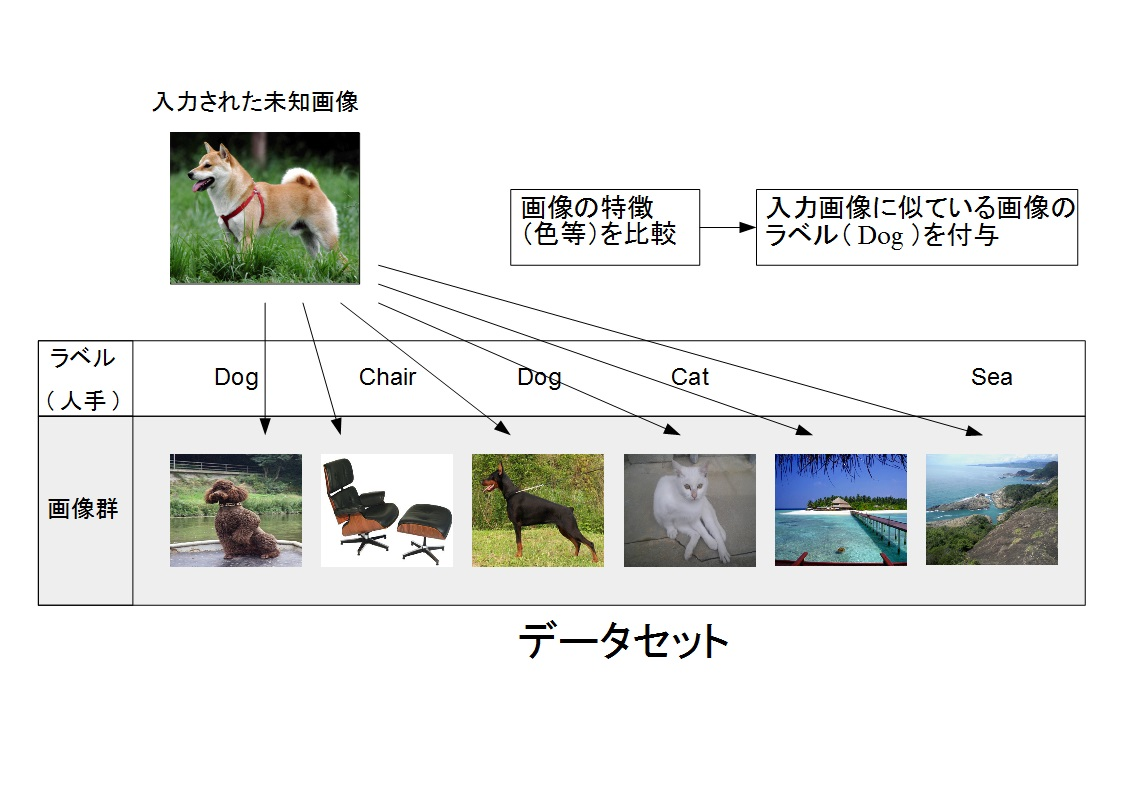
\includegraphics[scale=0.50]{gaiyou.jpg}
 \end{center}
 \caption{一般的な画像アノテーション手法の概要}
 \label{fig:abst}
\end{figure}

まず第一段階として,画像を収集して
各画像にラベルまたはタグと呼ばれる画像の内容を表すテキストを付与する.
このラベルは人間が手動で記述する場合もあるが,
Web上の周辺テキストを伴った画像を使うことで自動推定する場合もある.
それらラベルを付けた画像の特徴を統計的に分析することで,ラベルの持つ特徴を学習する.
次に第二段階として,未知の画像を入力し,その画像特徴と類似する画像群が共通して持つラベルを見つけ,
入力画像にそのラベルを付与する.
この様にして入力された画像の内容を推測するのが画像アノテーションである.

% 本稿では,画像の分類手法に工夫をこらし,入力画像に対するラベル付与の精度を高めるための実験を行った.
自動画像アノテーションの分野における研究課題としては,
画像の収集や画像へのラベル付与を自動化することで,
大規模な画像データセットの構築にかかる時間と労力を減らす課題がある.
%\section{画像アノテーション}
%
%前節で
%ラベル付与の自動化・高精度化の手法が研究されていると述べた.
それらの研究の中でも近年頻繁に研究されているものが,画像のブロブ化である.
ブロブ化は各画像を複数の領域に分割し,隣接する領域との特徴の差異を見ることで画像全体を分解することで行う.
これによって得られたブロブは,画像に写っている物体ごとに分割されている可能性が高いので,
注目しているブロブ以外の物体の有無に左右されることなく,そのブロブに対する精確なラベル付与が可能となる.
このブロブ化をデータセット内の全ての画像に施すことで,高精度の画像アノテーションを実現する.

Duygulu\cite{duygulu}らやJeon\cite{jeon}らは,すべての画像はブロブ(画像内の物体の塊)に単語を割り当てることで
内容物を記述することができるという前提で研究を行った.
JeonはDuyguluらの研究を元に,まずブロブと単語の同時分布を予習するためにCMRM(Cross-Media Relevance Model)を開発し,
更にそのモデルを改良した3つのモデルを開発した.
これらは画像を収集する際に自動で画像アノテーションを行う確率的生成モデルである.
その結果,Duyguluらが論文で公開した確率的生成モデルの画像アノテーションの平均精度0.20に比べ,
ほぼ倍の0.41という平均精度を示し,再現率についてもはるかによい結果となった.

またこれらの研究とは別のアプローチで画像アノテーションの精度向上を目指した研究がある.
渡邉ら\cite{watanabe}は,大規模Web画像データベースと
類似画像検索技術を用いた自動画像アノテーションシステムを実装した.
このシステムは,与えられた画像をクエリとして類似画像検索を行い,
検索結果の画像に付随するテキスト中の単語を確率的指標により評価することで,
特別な事前学習なしに画像を意味付けるキーワードを推定可能であることを示した.
このシステムを用いて5カテゴリ30概念の画像に対するアノテーションを行った結果,
10位内正解率がカテゴリ平均で43~75\%,全概念の平均で約59.1\%であった.

\section{テキスト処理}

Web上の周辺テキストを伴った画像から画像の内容を推定するのが画像アノテーションであるとみなすこともできる.
画像アノテーションの研究は多く存在する.
しかしテキスト処理として英語のテキスト処理を行うものが大部分である.
日本語の周辺テキストを処理する先行研究は発見することが出来なかった.
本研究では日本語テキスト処理を使った画像アノテーションの研究を行う.
%
ここでは
画像アノテーションを行うために
英語のテキスト処理と日本語のテキスト処理でどのような差があるのか
関連研究から推測する.

テキストの中の特定の対象を分類する様な問題の1つとしてposタガーがある.
英語のposタガーの性能は約8割程度の精度であることが報告されている
\cite{BirdKleinLoper09}
%,Ibanez:2011:EPS:1964799.1964819
.
日本語のposタガーの性能は約9割程度の精度であることが報告されている\cite{UniDicJp2010}.
この結果はベンチマークや学習データの違いによって変わることがあるため単純に比較することはできないが,
日本語テキスト処理の方が英語テキスト処理よりも精度が高い可能性を示している.
このことから周辺テキストが日本語の場合は,周辺テキストが英語の場合よりも高い精度で
画像アノテーションを実現できる可能性がある.
posタガーは単語の並んだ順番を処理する技法でもある.
このことから日本語の適当な手がかり表現を利用する手法は特に高い精度を達成できる可能性がある.

渡邉ら\cite{watanabe}の英語周辺テキストを利用した画像アノテーションの研究では,単純に単語の出現頻度を利用していた.
本研究では日本語の手がかり表現を利用した分類を行う.



%\chapter{類似画像検索とテキスト検索を用いた自動画像アノテーション}
\chapter{提案手法}
\label{sec:way}

%\section{概要}
ここでは本研究で提案する自動画像アノテーション手法を説明する.
図\ref{fig:way}に提案手法の概要を示す.
%
\begin{figure}[tb]
 \begin{center}
  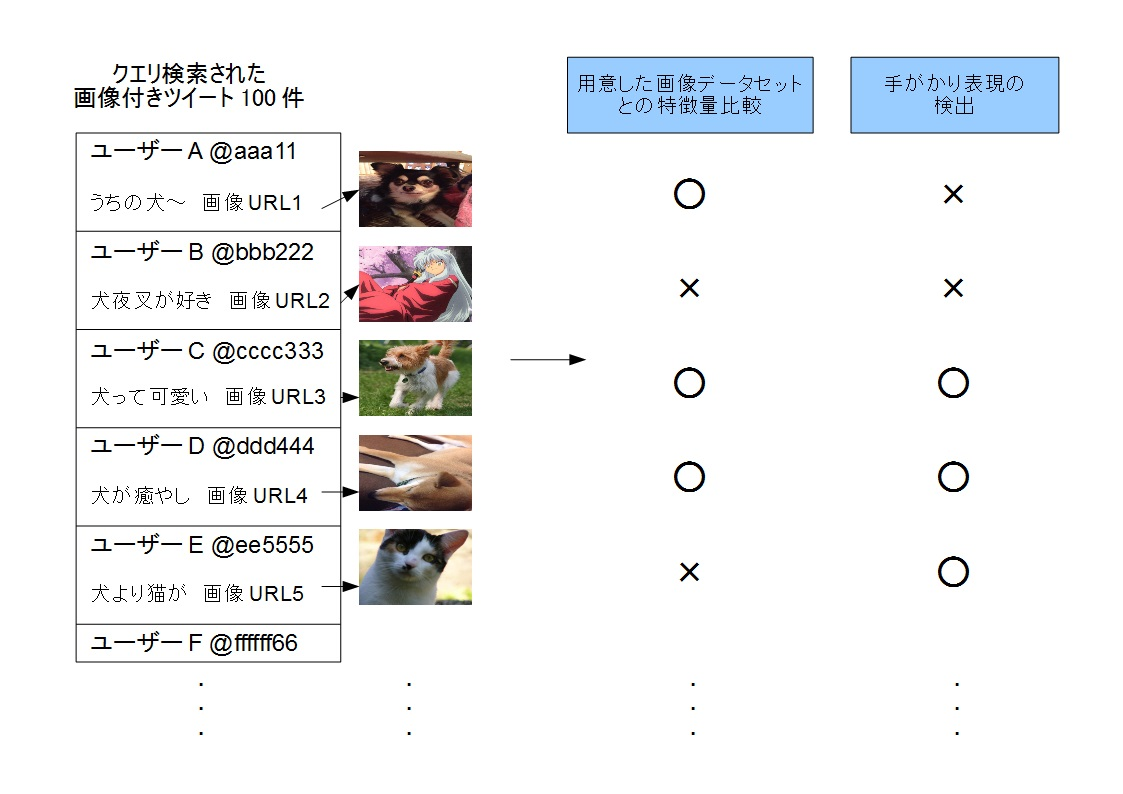
\includegraphics[scale=0.50]{way.jpg}
 \end{center}
 \caption{提案手法の概要}
 \label{fig:way}
\end{figure}
%
提案手法は,ツイート収集,類似画像検索,テキスト検索の3段階から構成される.


%Webから得られた画像と周辺テキストを収集する前処理と,
%類似画像検索とテキスト検索を用いて得られた画像を分類する処理に分けられる.

最初のツイート収集処理においては,TwitterAPIを利用し,認識したい物体名をクエリに指定して検索を行い,得られたツイートを収集する.
収集したツイートに付随するURLから,Twitterの公式アップローダにアップロードされた画像をそれぞれ取得する.

次の類似画像検索処理においては,まずユーザが手作業でクエリとして選んだ物体を表す参考画像を一枚,事前に用意する.
参考画像とは,クエリを正しく表していると実験者が判断し,類似画像検索の比較元とする画像である.
この参考画像をクエリとして,収集した画像群から類似画像を選別する.
ここで類似画像とは,クエリとした画像と色や形状などの特徴が近い画像のことである.
本研究では参考画像の色ヒストグラムの分布と類似した色ヒストグラムを持つ画像を類似画像とした.
この結果,参考画像と見た目の類似した画像が得られる.
%参考画像の選別は人手で行う必要があるが,ImageNetを使って自動化することも出来る.
%しかしこの自動化の処理の実装は今後の課題である.

最後のテキスト検索処理においては,選別された画像に伴うツイート本文に
手がかり表現を用いてさらに選別を行う.
この手がかり表現とは,選別された画像に付随するテキストが何を表しているかの手がかりとなる表現のことである.
ツイート本文中からその表現を検索することで,
そのツイートに付随する画像がクエリを正しく表現しているか否かの分類が行える.

この3つの処理を組み合わせ自動画像アノテーションを実現している.
類似画像検索処理とテキスト検索処理では異なる分類結果が与えられる.
%どちらか片方の処理で正解と分類された結果を正解とする論理和処理の結果が提案手法である.
以下では,ツイート画像収集と,類似画像検索,テキスト検索について詳細に説明する.

\section{ツイート画像収集}
\label{sec:tweetCollect}
TwitterAPI1.1の機能を使い,検索したい画像の名称をクエリとし,Twitterからツイートを検索する.
この際,オプションとして " -RT filter:images" をクエリに含める.
"-RT" は重複したツイートを取得することを避けるために追加した.
"filter:images" はTwitterの公式アップローダにアップロードされた画像のみを参照するために使用した.

次に収集した各ツイートから最後尾にあるURL部分を抜き出し,URL先からソースを入手する.
このソースから,正規表現でツイッターの公式アップローダに格納されている画像URLを抜き出し,
画像データをコピーして自機に保存することで画像群を収集することが可能である.
この処理の際,ツイートしたユーザーが許可のない他者からツイート情報にアクセス出来ないようにしたり,
ツイートを消去することによって,
収集したツイートのページや画像が格納されているアップローダのURLにアクセスできない場合がある.
この場合これらのツイートは無視し,画像が正常に保存できたツイートのみを改めてデータベースに格納する.
これらの処理によって,収集したツイートと,ツイートに対応した画像のデータベースが作成できる.


\section{類似画像検索}
\label{sec:similar}
提案手法では,各色が画像中に何ピクセルあるかを数えた色ヒストグラムの分布を画像の特徴量として扱い,
この分布が参考画像と類似している画像を類似画像として選別した.
色ヒストグラム処理の実装は
\url{http://aidiary.hatenablog.com/entry/20091003/1254574041}
で公開されているプログラムを参考に実装した.

色ヒストグラムは各色8ビットをそのままで計算すると16,777,216次元ベクトルとなり
計算にかかる時間が非常に大きくなる.
提案手法では各色を4分割した64色に減色した上でヒストグラムを算出する.
8ビットを4分割した2ビット,つまり0から3までを色番号として
%各番号は分けられた
代表値(0から63の場合は中心の32)の値に分類した.
例として
64色に減色した画像と,
その色ヒストグラムの棒グラフを
図\ref{fig:color}に示す.
%
\begin{figure}[tb]
 \begin{center}
  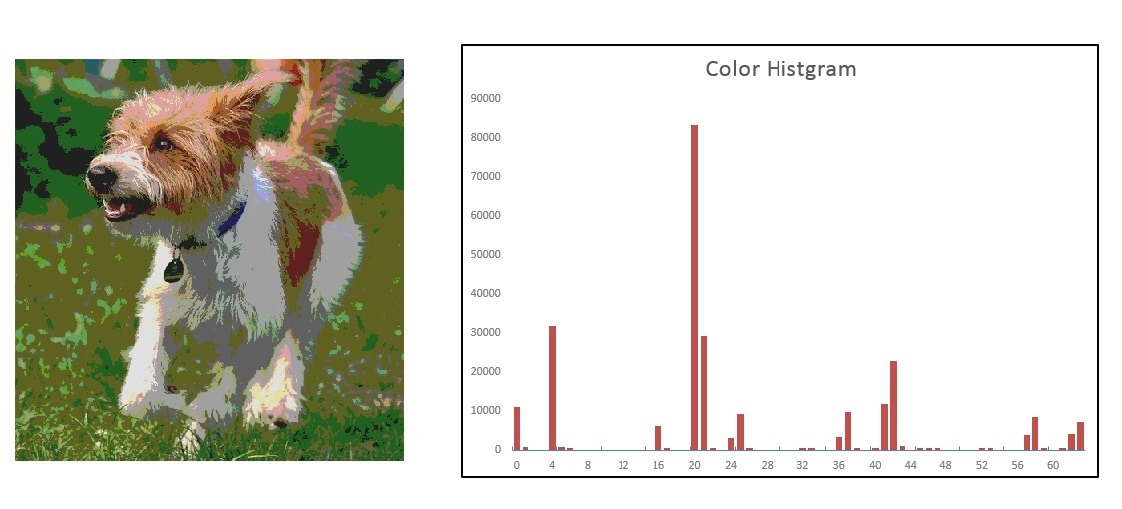
\includegraphics[scale=0.50]{colorhist.jpg}
 \end{center}
 \caption{色ヒストグラムの例}
 \label{fig:color}
\end{figure}
%
%
%OpenCVの色ヒストグラム類似度計測関数のドキュメントに色ヒストグラムを使う手法の詳細や参考文献が書いてあったはずなので色ヒストグラム処理の話を追加してください
図\ref{fig:color}左の犬の画像は
RGB値がそれぞれ32,96,160,224の4通りしかない.
各画素の色の種類は64色であるため,棒グラフの横軸は64個になっている.
横軸のビンの値は以下の式で表される.
\begin{eqnarray}
\mbox{bin} = (16 * R) + (4 * B) + G
\end{eqnarray}
このときR,G,Bの値はそれぞれの色番号である.
例えば
図\ref{fig:color}右の棒グラフで
最も値の高いbin=20は(R,G,B)=(1,1,0)であり,
画像中で濃い黄緑が
広い面積をとっていることがわかる.

本手法では,取得した画像群から
参考画像と類似した画像を選別する.
そのため,クエリ対象を正しく表している
参考画像を事前に人手で選別しておかなければならない.
この処理はImageNetを使って自動化することも出来るが
ImageNetで分類されたカテゴリにない対象も多くある.
例えば犬の画像はImageNetから自動で収集できるが,
\ref{sec:experiment}章の実験でクエリ対象とした柴犬のカテゴリはImageNetには存在しない.
この様な場合もあるため本実装では参考画像の選別は手動処理としている.
%
選別された参考画像と収集した画像群は全て同じサイズ(320*240)のJPEG形式に変換する.
これは色ヒストグラムを算出する際に,全ての画像において画素の記述方法を統一するためである.
次に,\ref{sec:tweetCollect}節で収集した画像と参考画像を減色した画像の色ヒストグラムを算出し,
それぞれのデータを作成する.

次に参考画像のヒストグラムデータをクエリとして,
Histogram Intersection
の考え方を使って
類似度を算出する.
Histogram Intersectionとは
2つの色ヒストグラム
$H_1,H_2$
が与えられたときの類似度を
以下の式で与える手法である.
%
\begin{eqnarray}
\mbox{Similarity} = \frac{\sum_{i=0}^{63} min(H_1[i],H_2[i])}{\sum_{i=0}^{63} H_1[i]}
\end{eqnarray}
%
ここで$H_k$は$k$番目の画像の色ヒストグラムであり,
$H_k[i]$はそのヒストグラムの$i$番目のビンの値である.
%このとき2つのヒストグラムをH1,H2,ヒストグラムHのi番目のビンの値をH[i]と定義する.
この類似度は正規化がなされているため,値は0.0から1.0となり,
2つのヒストグラムが似ているほど大きな値をとる.
この類似度が設定した閾値を超えた画像を,クエリを表している画像として分類する.
%%%%%%%%%%閾値が明確に決められない場合にROCカーブを描いて性能を比較する場合も%%%%%%%%%%%%
%%閾値を 0 から1まで 0.01 ずつ大きくしていき,それぞれの閾値において類似画像検索の適合率と再現率を求める.%%



\section{テキスト検索}
\label{sec:textSearch}
\ref{sec:tweetCollect}節で
収集したツイートの本文から手がかり表現を見つけ,そのツイートの持つ画像を分類する.

\subsection{手がかり表現集合の収集}
本手法で使用する手がかり表現は以下の手順で得る.
まずTwitterから収集した画像付きツイートから,正しく画像の内容に言及しているツイートのみを人手で選別する.
選別したツイート群を言語処理にかけ,それぞれのツイートから動詞と形容詞を抽出する.
抽出した単語から重複をなくした集合を手がかり表現の集合とみなし,画像分類に用いる.
なお,本手法で使用した手がかり表現の集合を得るために使用したツイートは,
\ref{sec:examination}章で使用した複数のカテゴリのツイートを収集した際,
評価実験に使用しなかった一部のツイートから分類した合計100件のツイートである.
また言語処理には形態素解析エンジンMecab
(\url{http://mecab.googlecode.com/svn/trunk/mecab/doc/index.html})のver0.996を使用し,
ツイート中から分割された単語のうち品詞が動詞と形容詞のもののみを抽出したものを使用している.

抽出した手がかり表現の一部を表\ref{tab:predicate}に示す.

\begin{table}[bt]
\begin{center}
\caption{抽出された手がかり表現の一部}
\label{tab:predicate}
\begin{tabular}{|l|r|r|r|}\hline
動詞& 撮っ,佇む,持っ,する,たつ,吠え,飼い,笑っ,寝,見つかり,似,etc \\ \hline
形容詞& かわいい,よい,近かっ,ほしい,可愛い,人懐っこく,可愛,すっごい,etc \\ \hline
\end{tabular}
\end{center}
\end{table}

\subsection{ツイート文の解析}

収集したツイートを1文ずつMecabにかけ,
手がかり表現の集合に含まれる単語がそのままの形でツイート文に含まれているか1つずつ調べ,
1ツイート中に合計3つ以上の単語を含んでいるツイートの持つ画像は,
クエリとして選んだ物体を表していると判断した.
この3という数は,抽出に使用したツイート1文から抽出できた動詞,形容詞の数の平均を採用した.

\chapter{評価実験}
\label{sec:experiment}
\section{データセット}

評価実験として提案手法で柴犬の画像を分類する実験を行い,分類結果の精度評価を行った.
%本稿では,Twitterに投稿された画像付きツイートを収集し,データとして用いた.
参考画像としてwikipedia(\url{http://ja.wikipedia.org/})の柴犬の記事にある画像を使用した.
データは2015年1月27日に,"柴犬 -RT filter:images"をクエリとして
\label{sec:tweetCollect}節で紹介したようにツイートを収集し,
その結果として得られた3462件のツイートと画像を収集した.
これらのツイートと画像に参考画像を加えたものをデータセットとする.
このデータ群を提案手法でアノテーションすることで得られた最終的な分類結果の画像に,
どれだけ柴犬の画像が含まれているかを人手で評価し,適合率を算出した.
適合率は類似画像検索の分類結果に含まれる正解データの割合である.
同様に,wikipediaのシャム猫の記事にある画像を参考画像として,
"シャム猫 -RT filter:images"をクエリとして得られた932件のツイートと画像を提案手法で分類し,
その分類結果の精度評価を行った.
%これらのツイートと画像をデータセットとした.

\section{実験結果}
\label{sec:expresult}

本手法による結果を人手で分類し,画像分類精度を評価した結果を表\ref{tab:result-shiba}に示す.
なお取得数と分類結果の単位はいずれも枚である.

まずデータセットの柴犬の画像3462枚とシャム猫の画像932枚に対し,
各画像の色ヒストグラムデータを作成し,参考画像と比較して類似度を算出する.
求めた類似度が設定した閾値を上回る画像を,クエリを表している画像として分類する.
このとき閾値を0.58とした.
この閾値は柴犬,シャム猫以外の対象に対して同様の実験を行い,うまくいく閾値を手動で選別することで決定した.
類似画像検索で柴犬の画像であると判断した画像は1338枚,シャム猫の画像であると判断した画像は430枚であった.

分類した画像に対応するツイートに対して\ref{sec:textSearch}節で説明したテキスト検索処理を行い,
条件を満たしたツイートに付随する画像を柴犬を表している画像として分類した.
この結果,柴犬の画像であると判断された画像は429件,シャム猫の画像であると判断された画像は159件となった.

\section{評価}

柴犬をクエリとして得られた429件の画像のうち,人手で柴犬を表していると判断できる画像は336件であった.
シャム猫をクエリとして得られた159件の画像のうち,人手で柴犬を表していると判断できる画像は132件であった.
つまり提案手法によって得られたトレーニングセットの適合率はそれぞれ約0.78,約0.83であり,
含まれる誤りの画像は2割程度であると判断できる.
これは\label{sec:related}節で述べた許容範囲内である3割を下回っており,トレーニングセットとして十分に機能するといえる.


\begin{table}[tb]
\begin{center}
\caption{提案手法によって分類された柴犬とシャム猫の画像トレーニングセット精度}
\label{tab:result-shiba}
\begin{tabular}{|l|r|r|r|r|}\hline
& 取得数& 分類結果& 正解数& 適合率(\%) \\ \hline \hline

柴犬& 3462& 429& 336& 0.78 \\ \hline
シャム猫& 932& 159& 132& 0.83 \\ \hline
\end{tabular}
\end{center}
\end{table}

\chapter{考察}
\label{sec:examination}

\ref{sec:expresult}節で述べたように,
柴犬をクエリにして得られた画像3462枚を提案手法で分類した結果,得られた画像数は429件となった.
しかし本手法の各手順で,柴犬を表しているのに柴犬の画像ではないと判断されてしまった画像もある.
この章では提案手法のうち2つの分類処理やその組み合わせが適切かどうか考察する.

\section{考察実験}
\subsection{データセット}

データの収集は2015年1月27日に,"[カテゴリ名] -RT filter:images"をクエリとして
犬,猫,狐,椅子,メインクーンのツイートを収集し,
収集したツイート中から無作為にそれぞれ300件ずつツイートを選び,対応する画像を取得した.
ただしメインクーンについてはクエリを含むツイート数が少なく,
192件しか取れなかった.
犬,猫,狐はある程度大きなカテゴリの中で,ツイッターに画像がありそうなものを選んだ.
椅子は動物以外での分類精度を確かめるために選んだ.
メインクーンは評価実験に使用した柴犬やシャム猫と同程度の広さのカテゴリの結果を知るために選んだ.

取得できたツイートと画像に参考画像を加えたものを,各カテゴリのデータセットとする.
収集した画像を人手で判別しておき,各分類手法でどれだけの適合率で画像を分類できたかを評価する.
この際,クエリが動物であればその動物の顔が半分以上見えていれば正解とした.
またクエリが椅子の場合は,人や物などの障害物があってもいいので,
椅子のほぼ全体が画像内に収まっているものを正解とした.
なお評価する手法は類似画像検索のみ(1),テキスト検索のみ(2),類似画像検索とテキスト検索の和(1∪2),
提案手法である類似画像検索とテキスト検索の積(1∩2)の分類の4手法である.

\subsection{実験結果}

各カテゴリをクエリとして得られたツイートと画像を各分類にかけた結果を以下に示す.

犬で得られた画像を人手で分類した結果,300枚中130枚が正解と判別できた.
(1)では50枚の画像を分類し,そのうち32枚の正解を含んでおり,適合率は0.640であった.
(2)では195枚の画像を分類し,そのうち87枚の正解を含んでおり,適合率は0.446であった.
(1∪2)では222枚の画像を分類し,そのうち103枚の正解を含んでおり,適合率は0.464であった.
(1∩2)では23枚の画像を分類し,そのうち16枚の正解を含んでおり,適合率は0.696であった.

猫で得られた画像を人手で分類した結果,300枚中105枚が正解と判別できた.
(1)では67枚の画像を分類し,そのうち39枚の正解を含んでおり,適合率は0.582であった.
(2)では172枚の画像を分類し,そのうち64枚の正解を含んでおり,適合率は0.372であった.
(1∪2)では199枚の画像を分類し,そのうち74枚の正解を含んでおり,適合率は0.372であった.
(1∩2)では40枚の画像を分類し,そのうち29枚の正解を含んでおり,適合率は0.725であった.

狐で得られた画像を人手で分類した結果,300枚中7枚が正解と判別できた.
(1)では42枚の画像を分類し,そのうち4枚の正解を含んでおり,適合率は0.095であった.
(2)では186枚の画像を分類し,そのうち3枚の正解を含んでおり,適合率は0.016であった.
(1∪2)では198枚の画像を分類し,そのうち4枚の正解を含んでおり,適合率は0.020であった.
(1∩2)では30枚の画像を分類し,そのうち3枚の正解を含んでおり,適合率は0.100であった.

椅子で得られた画像を人手で分類した結果,300枚中149枚が正解と判別できた.
(1)では92枚の画像を分類し,そのうち46枚の正解を含んでおり,適合率は0.500であった.
(2)では180枚の画像を分類し,そのうち74枚の正解を含んでおり,適合率は0.411であった.
(1∪2)では211枚の画像を分類し,そのうち101枚の正解を含んでおり,適合率は0.479であった.
(1∩2)では31枚の画像を分類し,そのうち19枚の正解を含んでおり,適合率は0.613であった.

メインクーンで得られた画像を人手で分類した結果,192枚中142枚が正解と判別できた.
(1)では17枚の画像を分類し,そのうち15枚の正解を含んでおり,適合率は0.882であった.
(2)では111枚の画像を分類し,そのうち86枚の正解を含んでおり,適合率は0.775であった.
(1∪2)では119枚の画像を分類し,そのうち92枚の正解を含んでおり,適合率は0.773であった.
(1∩2)では9枚の画像を分類し,その全てが正解であり,適合率は1.000であった.

実験結果の再現率,適合率,F 値をまとめたものを表\ref{tab:result-ex}に示す.
ここで,再現率は人手で判定したクエリを表す画像のうち実際に分類できていた正解データ画像の割合である.
さらに,求めた再現率および適合率から F 値を算出する.
F 値($F\verb|-|measure$)は適合率($precision$)と再現率($recall$)の調和平均であり,次式で求める.

\begin{eqnarray}
F\verb|-|measure = \frac{2・precision・recall}{precision+recall}
\end{eqnarray}

%類似画像検索,テキスト検索,二手法の組み合わせによる画像分類の結果を表\ref{tab:result}に示す.

\begin{table}%[tb]
\begin{center}
\caption{各カテゴリの分類における再現率,適合率,F値}
\label{tab:result-ex}
\begin{tabular}{|l|r|r|r|r|}\hline
&& 再現率& 適合率& F値\\ \hline \hline
犬
& 類似画像検索(1)& 0.246& 0.640& 0.356 \\ \cline{2-5}
& テキスト検索(2)& 0.669& 0.446& 0.535 \\ \cline{2-5}
& 提案手法(1∪2)& 0.792& 0.464& 0.585 \\ \cline{2-5}
& 提案手法(1∩2)& 0.123& 0.696& 0.209 \\ \hline
猫
& 類似画像検索(1)& 0.371& 0.582& 0.453 \\ \cline{2-5}
& テキスト検索(2)& 0.610& 0.372& 0.462 \\ \cline{2-5}
& 提案手法(1∪2)& 0.705& 0.372& 0.487 \\ \cline{2-5}
& 提案手法(1∩2)& 0.276& 0.725& 0.400 \\ \hline
狐
& 類似画像検索(1)& 0.571& 0.095& 0.163 \\ \cline{2-5}
& テキスト検索(2)& 0.429& 0.016& 0.031 \\ \cline{2-5}
& 提案手法(1∪2)& 0.571& 0.020& 0.039 \\ \cline{2-5}
& 提案手法(1∩2)& 0.429& 0.100& 0.162 \\ \hline
椅子
& 類似画像検索(1)& 0.309& 0.500& 0.382 \\ \cline{2-5}
& テキスト検索(2)& 0.497& 0.411& 0.450 \\ \cline{2-5}
& 提案手法(1∪2)& 0.678& 0.479& 0.561 \\ \cline{2-5}
& 提案手法(1∩2)& 0.128& 0.613& 0.211 \\ \hline
メインクーン
& 類似画像検索(1)& 0.106& 0.882& 0.189 \\ \cline{2-5}
& テキスト検索(2)& 0.606& 0.775& 0.680 \\ \cline{2-5}
& 提案手法(1∪2)& 0.648& 0.773& 0.705 \\ \cline{2-5}
& 提案手法(1∩2)& 0.063& 1.000& 0.119 \\ \hline
\end{tabular}
\end{center}
\end{table}

\subsection{各カテゴリの分類結果の特徴}
犬と猫の2カテゴリにおいては分類結果の偏りが非常に似ている.
しかし,狐のカテゴリでは収集した画像に狐が写っている画像が極端に少なく,
その分類結果はまともに評価できなくなっている.
これは狐が身近にいる動物ではないため,狐の姿を表す画像が少なく,
代わりにイラストが多く含まれていたことが理由としてあげられる.
椅子のカテゴリの分類結果は,全体的に犬や猫より悪い結果となっている.
これは,椅子を表すツイートにおいて動詞や形容詞があまり使われておらず,
抽出された手がかり表現の集合にも椅子に適した表現が少なかったことがあげられる.
メインクーンのカテゴリにおいては,カテゴリの広さが狭いため,
収集できた画像中に含まれる正解データが多めとなっている.
このため,メインクーンの分類の適合率は全体的に高くなっている.

\subsection{類似画像検索による画像分類精度評価}
類似画像検索の分類精度は,全体的に再現率が低く,適合率が高い傾向にある.
適合率が高いのは参考画像を人手で選択するので確実に正解の画像を選ぶことができるため,
類似画像検索では正解に近い色の分布を持つものしか分類しないからである.
逆に,再現率が低いのは,分類する数が少ないため,
その中に含まれる正解データも必然的に少なくなることが理由である.
また設定した閾値も0.58と高めであるため,犬,猫,狐では分類結果の画像数も300中約50とかなり少ない.
またメインクーンの分類結果が少ない理由は,分類されていない画像を見るに,
毛色や撮る状況によって,色の分布が他の動物より大きく左右されているためであると推測できる.
改良案としては,類似画像検索に使う閾値を分類するカテゴリごとに分けることや,
類似画像検索に使用する特徴量を変えることがあげられる.

\subsection{テキスト検索による画像分類精度評価}
テキスト検索の分類は,基本的に多めの画像を分類している.
これは,手がかり表現の集合に基本的な動詞などが含まれているため,
多めのツイートが分類条件に当てはまっていると推測できる.
全体的に再現率が高く適合率が少し低めとなっている傾向にある.
しかし猫,犬,椅子を分類した結果のF値は0.5付近と精度がいいとはいえず,
ここに大きな改良の余地が残されていると思われる.

\subsection{2手法の組み合わせによる画像分類精度評価}
類似画像検索とテキスト検索,2手法の和の組み合わせでは,
狐以外の全カテゴリにおいて1つの手法による分類結果よりF値が高くなっている.
これは,分類された画像の量が増えた以上に,その結果に含まれる正解データの数が増えたためである.
反面,分類結果には多くの間違いも含まれており,
量を除いてトレーニングセットとして使えそうな分類結果には至っていない.

しかし,2手法の積の組み合わせではF値が極端に低く分類結果の量が少ない代わりに,
その中に含まれる正解データの割合は非常に高くなっている.
犬や猫は7割近い適合率を持ち,それらに劣る椅子の結果でも6割の適合率を持っている.
これらのことから,現状の2手法の組み合わせとしては積の組み合わせが有用であることがわかる.
しかし,分類の結果得られた画像の量はかなり少なくなっている.

この手法を使用した提案手法では多くのツイートを取得したため,
トレーニングセットとして利用するのに十分な画像量となったが,
狐のように正解の画像の量が少なくなることが予想される
身近に居ない動物の画像は収集してもトレーニングセットとして使用できないと思われる.
反面,今回の目的のような狭い範囲のカテゴリにおける画像分類には,
現在の手法でも数回収集を繰り返すことで十分に利用できることがわかる.
